\documentclass[letterpaper,11pt]{article}
\oddsidemargin -1.0cm \textwidth 17.5cm

\usepackage[utf8]{inputenc}
\usepackage[activeacute,spanish, es-lcroman]{babel}
\decimalpoint
\usepackage{amsfonts,setspace}
\usepackage{amsmath}
\usepackage{amssymb, amsmath, amsthm}
\usepackage{comment}
\usepackage{float}
\usepackage{amssymb}
\usepackage{dsfont}
\usepackage{anysize}
\usepackage{multicol}
\usepackage{enumerate}
\usepackage{graphicx}
\usepackage[left=1.5cm,top=2cm,right=1.5cm, bottom=1.7cm]{geometry}
\setlength\headheight{1.5em} 
\usepackage{fancyhdr}
\usepackage{multicol}
\usepackage{hyperref}
\usepackage{wrapfig}
\usepackage{subcaption}
\usepackage{siunitx}
\usepackage{cancel}
\usepackage{mdwlist}
\usepackage{svg}
\pagestyle{fancy}
\fancyhf{}
\renewcommand{\labelenumi}{\normalsize\bfseries P\arabic{enumi}.}
\renewcommand{\labelenumii}{\normalsize\bfseries (\alph{enumii})}
\renewcommand{\labelenumiii}{\normalsize\bfseries \roman{enumiii})}


\begin{document}

\fancyhead[L]{\itshape{Facultad de Ciencias F\'isicas y Matem\'aticas}}
\fancyhead[R]{\itshape{Universidad de Chile}}
\rfoot[]{pág. \thepage}

\begin{minipage}{11.5cm}
    \begin{flushleft}
        \hspace*{-0.6cm}\textbf{FI1000 Introducción a la Física Clásica}\\
        \hspace*{-0.6cm}\textbf{Tutor:} Alejandro Cartes
    \end{flushleft}
\end{minipage}

\begin{picture}(2,3)
    \put(366, -10){
\includegraphics[scale=0.9]{2020-1/Imágenes/logo/dfi-fcfm.pdf}}
\end{picture}

\begin{center}
	\LARGE\textbf{Tutoría C3 - 2}\\
	\Large{Colisiones, Centro de Masa y Torque}
\end{center}

\vspace{-1cm}
\begin{enumerate}\setlength{\itemsep}{0.4cm}

\item[]

\item 
\begin{enumerate}
    \item Dos objetos pueden deslizar sin roce por un riel circular de radio $R$ colocado en un plano vertical, como se muestra en la figura \ref{fig1}. El objeto de masa $3m$ se coloca en la parte más alta del riel y se conecta a un extremo de un resorte ideal de constante elástica $k$ y largo natural nulo. El otro extremo del resorte se fija a un punto colocado a una distancia $2R$ del centro del riel en el eje horizontal. El objeto de masa $m$ se coloca en reposo en la parte más baja del riel.

    Al soltar el objeto de masa $3m$ del reposo, este se mueve por el riel para colisionar con el objeto de masa $m$, quedando adheridos. Calcule el valor de $m$ para que el par de objetos llegue justo hasta al punto $A$.


    \item Si ahora el material de los objetos y la configuración cambia, como se muestra en la figura \ref{fig2}. Determine el valor de $m$ que permite que el objeto de masa $3m$ llegue al punto A y el bloque de masa $m$ llegue al punto $B$, sin que sigan subiendo. Considere en este caso una colisión elástica.
\end{enumerate}

\begin{figure}[H]
    \centering
    \begin{subfigure}[t]{0.45\textwidth}
        \centering
        \svgpath{../../2023-1/img/TD 4}
        \includesvg[width=1\textwidth]{P1.svg}
        \caption{}
        \label{fig1}
    \end{subfigure}
    \begin{subfigure}[t]{0.35\textwidth}
        \centering
        \svgpath{../../2021-2/img/aux9}
        \includesvg[width=1\linewidth]{p3.svg}
        \caption{}
        \label{fig2}
    \end{subfigure}
\end{figure}

\item Un capitán de barco desea retirar una boya de masa desconocida. Cuando el barco se encuentra a una distancia $L$ de la boya, estando en reposo, se lanza una cuerda para atraparla. Al recoger la cuerda se logra subir la boya al barco, y el capitán mide que el barco se ha movido una distancia $d$ en dirección a la boya ($d<L$). Considerando que el barco posee una masa $M$, determine la masa de la boya.

\item 
\begin{multicols}{2} Una barra de masa $M$, distribuida homogéneamente, y largo $L$ se dobla en un ángulo $\alpha$ a una distancia $\lambda L$, con $\lambda \leq 1/2$. La estructura se encuentra en equilibrio gracias a una masa $m$ que se cuelga en uno de los extremos.
    \begin{enumerate}
        \item Determine la tensión $T$ y el valor de $m$
        
        \item ¿Cómo cambian sus resultados si la barra, en vez de estar doblada en un ángulo $\alpha$ hacia abajo, está doblada hacia arriba?
    \end{enumerate}
    
    \columnbreak
    
    \begin{figure}[H]
        \centering
        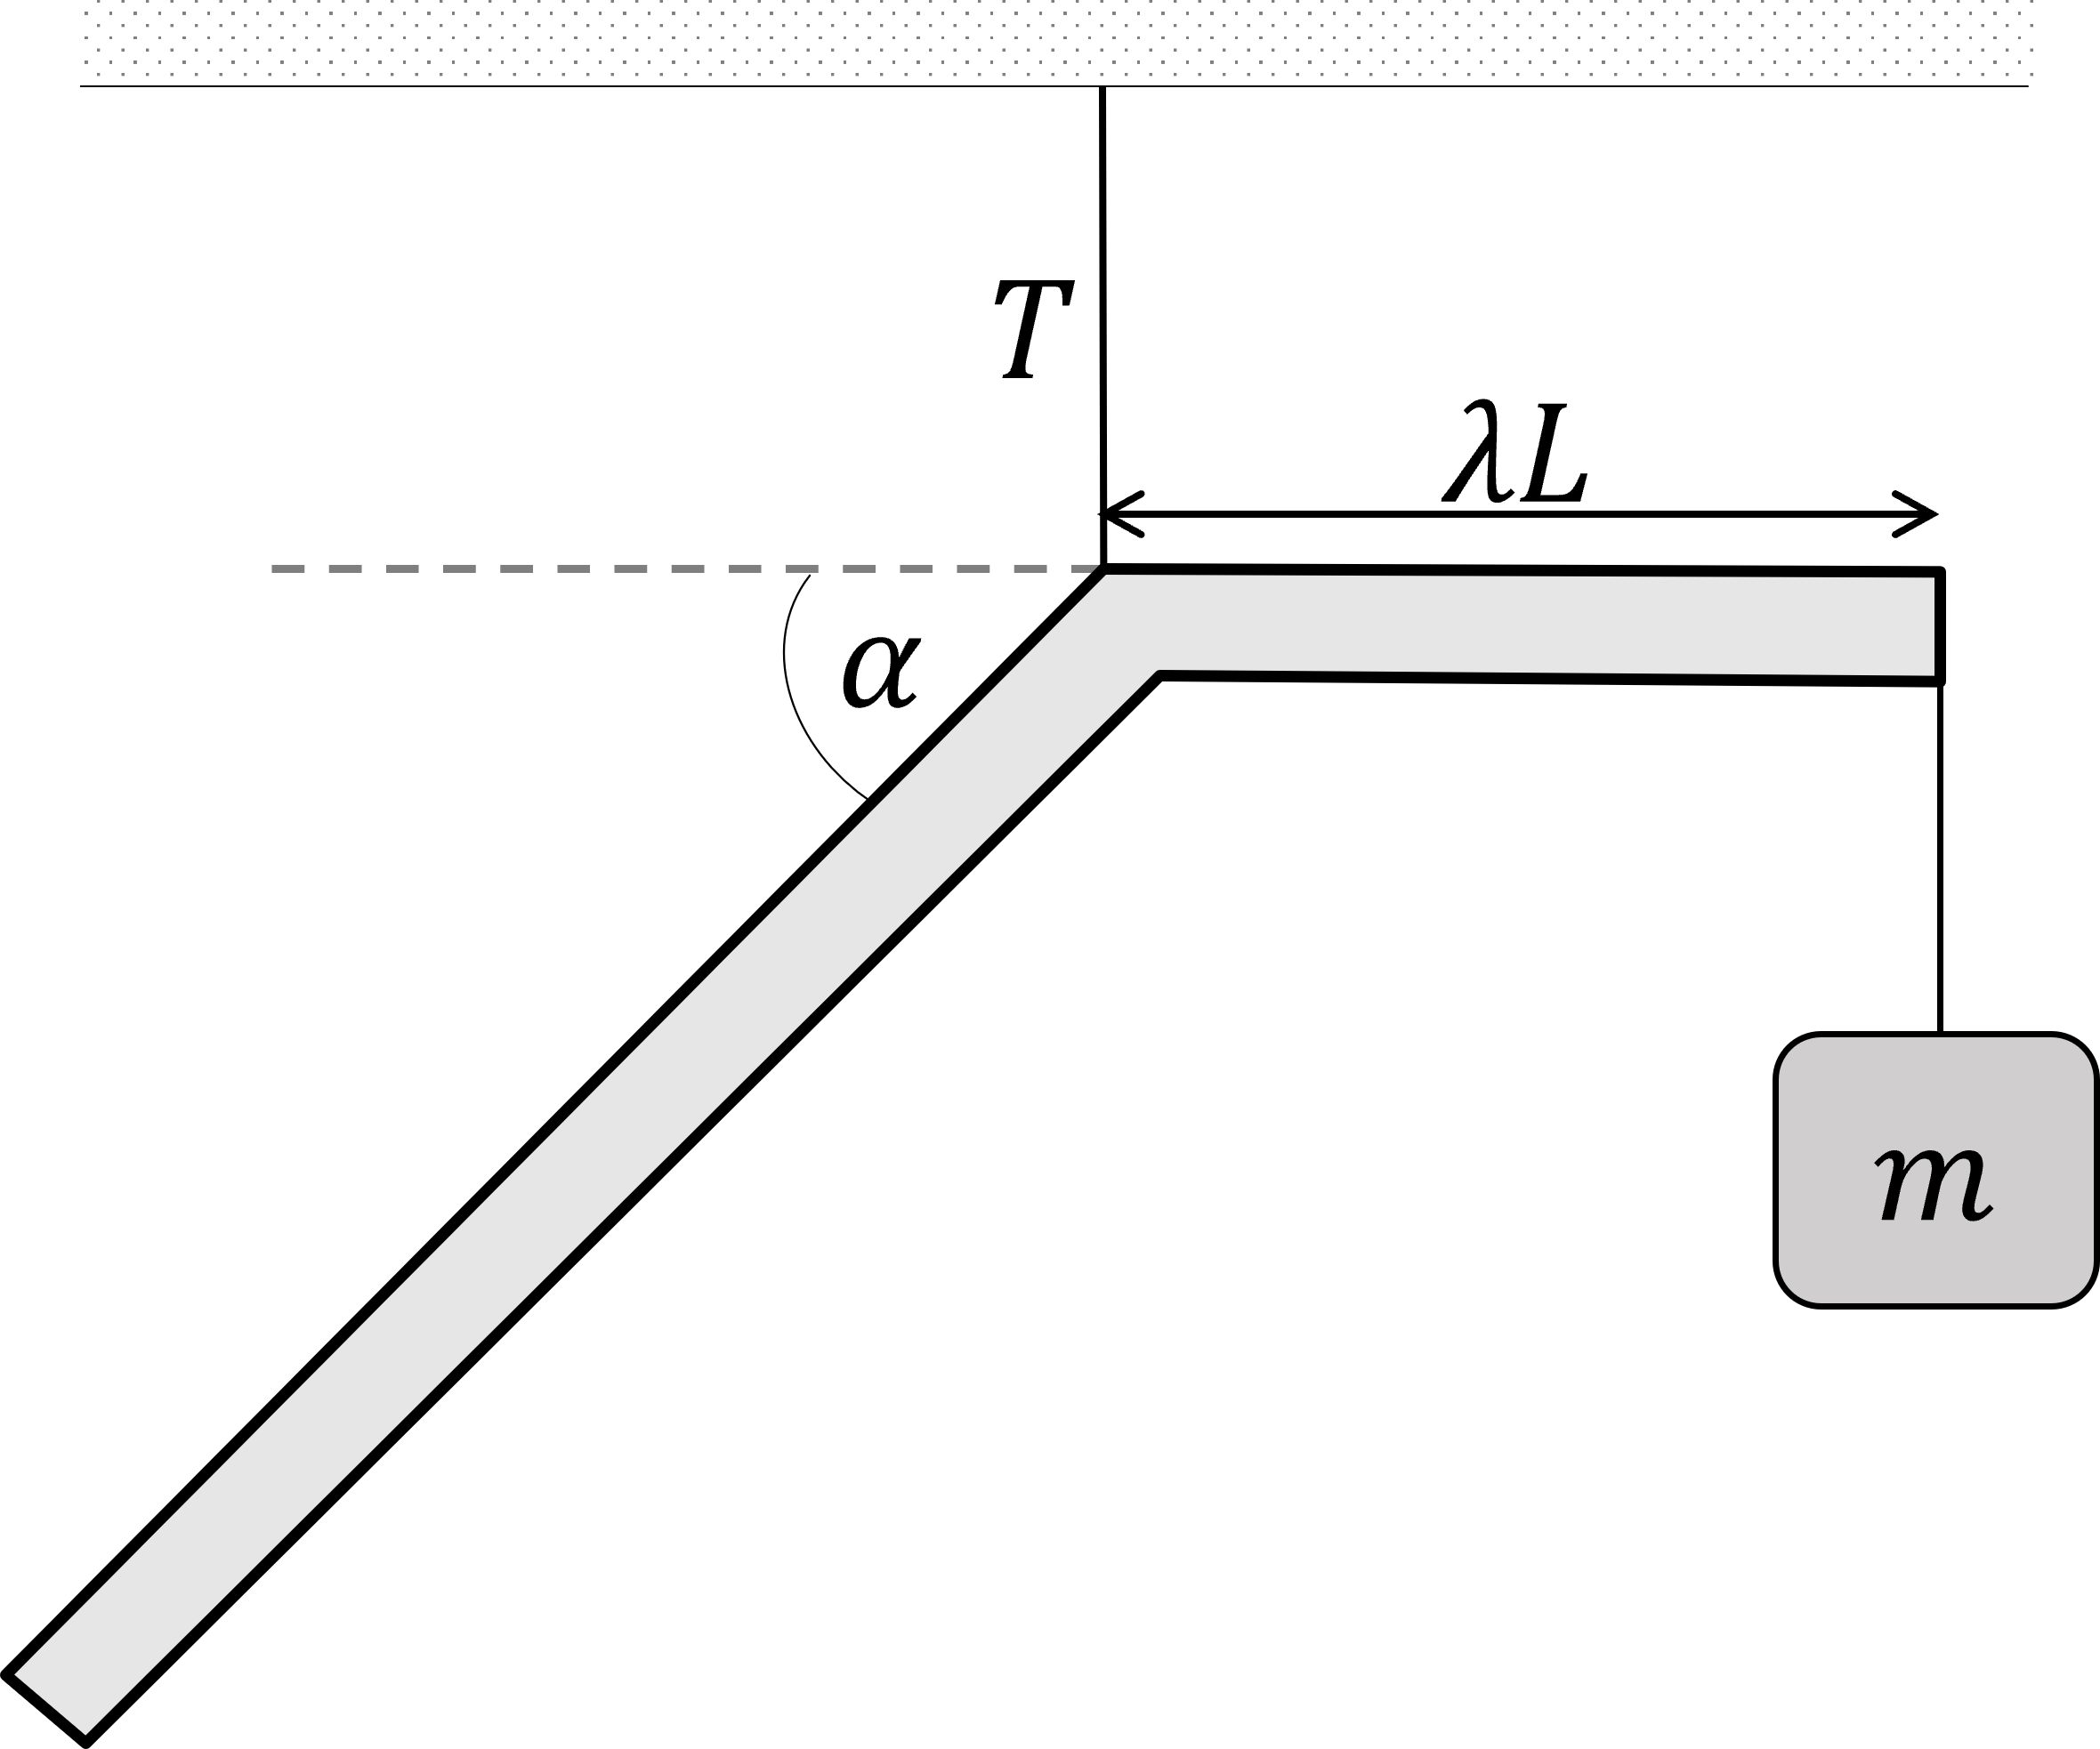
\includegraphics[width=0.6\linewidth]{2022-1/img/aux12/barra_dobla.png}
    \end{figure}
\end{multicols}

% Para imágenes vectoriales -> el texto tiene que estar en LaTeX
% \begin{figure}[htbp]
%   \centering
%   \svgpath{../Imagenes/ejercicios}  -> .. irse pa'trás 
%   \includesvg{ej5.svg}
% \end{figure}

\end{enumerate}
\end{document}